\section{测度论}

\begin{example}[Banach-Tarski 悖论]
    设 \(B^3\) 是单位球, 则存在 \(B^3\) 的一个分解, 使得可以用有限个刚体运动将其分解为两个 \(B^3\).

    \begin{proof}
        先去掉中心, 选取一过球心的半径为 \(1/3\) 的圆, 以 \(1\) 为单次旋转的弧度构造变换 \(\rho\),
        对 \(O := (0,0)\) 做变换得到 \(O,\rho O, \rho^2 O, \rho^3 O\), 可以将此列前移后移以去除生成零点.

        其次, 存在两个旋转 \(\alpha,\beta\) 使得其生成的 \(SO(3)\) 子群自由, 例如典范的选取:

        \[
            \alpha = \begin{pmatrix}
                \frac{1}{3} & - \frac{2 \sqrt{2}}{3} & 0 \\
                \frac{2 \sqrt{2}}{3} & \frac{1}{3} & 0 \\
                0 & 0 & 1
            \end{pmatrix}, \beta = \begin{pmatrix}
                1 & 0 & 0 \\
                0 & \frac{1}{3} & - \frac{2 \sqrt{2}}{3} \\
                0 & \frac{2 \sqrt{2}}{3} & \frac{1}{3}
            \end{pmatrix}
        \]

        则其任何 \(k\) 次变换总将 \((1,0,0)\) 映射为 \((a,b \sqrt{2},c)/3^k\) 且 \(b\) 不是 \(3\) 的倍数于是其生成的群自由,
        记一个这样的群为 \(G = \langle \alpha, \beta \rangle\).

        我们采取同样的技巧证明 \(B^3 \setminus \{O\}\) 可以分解合成为 \(E := \{x \in B^3:\forall g \in G \implies g x \neq x\}\),
        \(D\) 可数故 \(D\) 中两点中点亦可数, 存在一过 \(O\) 的轴线 \(L\) 使得 \(L\) 不过任意 \(D\) 中两点的中点, 取 \(\rho\) 为绕 \(L\) 旋转 \(1\) 的变换,
        则得到 \(B^3 \setminus E, \rho (B^3 \setminus E), \rho^2 (B^3 \setminus E), \cdots\), 消去得到 \(E\).

        对 \(E\) 做轨道分解并且选取代表元集 \(M\), 考察 \(f M\) 作为 \(E\) 的分解, 
        我们证明两个 \(F\) 可以合成为一个 \(F\), 首先选取第一个 \(F\) 以 \(\alpha\) 开头的元素,
        使其不动, 不以 \(\alpha\) 开头的元素, 使其乘上 \(\alpha^{-1}\), 对称的, 对第二个 \(F\) 和 \(\beta\) 做此操作,
        得到 \(F \setminus \{e\}\), 最后选取 \(\alpha\) 的幂级数 \(\{e,\alpha,\alpha^2, \cdots\}\) 向左平移即可.
    \end{proof}
\end{example}

此悖论意在说明在允许 \ref{axiom:NBG Axiom of Global Choice} 的情况下, 并非所有集合均可测.

\subsection{测度}

\subsubsection{代数}

\begin{definition}[代数]
    设 \(X\) 是一个集合, \(\mathcal{A} \subseteq \mathcal{P} (X)\) 是 \(X\) 的一个子集族, 如果满足

    \begin{enumerate}
        \item \(X \in \mathcal{A}\)
        \item \(A \in \mathcal{A} \implies X \setminus A \in \mathcal{A}\)
        \item \(A, B \in \mathcal{A} \implies A \cup B \in \mathcal{A}\)
    \end{enumerate}

    则称 \(\mathcal{A}\) 是 \(X\) 上的一个代数.
\end{definition}

\begin{definition}[\(\sigma\) - 代数]
    设 \(X\) 是一个集合, \(\mathcal{A} \subseteq \mathcal{P} (X)\) 是 \(X\) 的一个子集族, 如果满足

    \begin{enumerate}
        \item \(X \in \mathcal{A}\)
        \item \(A \in \mathcal{A} \implies X \setminus A \in \mathcal{A}\)
        \item \(A_1, A_2, \cdots \in \mathcal{A} \implies \bigcup_{i \in \mathbb{N}} A_i \in \mathcal{A}\)
    \end{enumerate}

    则称 \(\mathcal{A}\) 是 \(X\) 上的一个 \(\sigma\)-代数.
\end{definition}

\begin{remark}
    在此处 \(\sigma\) 表示可数, 同样表示可数的有 \ref{definition:sigma-locally finite family of topological space}.
\end{remark}

\begin{corollary}
    \(\sigma\)-代数是代数.
\end{corollary}

\begin{example}
    设 \(X\) 是一个集合, \(\mathcal{A} = \{\varnothing, X\}\), 则 \(\mathcal{A}\) 是 \(X\) 上的一个 \(\sigma\)-代数.

    设 \(X\) 是一个集合, \(\mathcal{A} = \mathcal{P} (X)\), 则 \(\mathcal{A}\) 是 \(X\) 上的一个 \(\sigma\)-代数.

    设 \(X\) 是一个集合, 其上所有有限集以及其补集构成的集合族是 \(X\) 上的一个代数, 但不总是 \(\sigma\)-代数.
\end{example}

\begin{lemma}
    给出 \(X\) 上 \(\sigma\) - 代数 \({(\mathcal{A}_i)}_{i \in I}\), 其交 \(\bigcap_{i \in I} \mathcal{A}_i\) 也是 \(\sigma\) - 代数,
    代数亦然.

    \begin{proof}
        逐条验证即可.
    \end{proof}
\end{lemma}

\begin{corollary}
    对于任意集族 \(\mathcal{F}\), 存在最小的 \(\sigma\)-代数 \(\sigma(\mathcal{F})\), 使得 \(\mathcal{F} \subseteq \sigma(\mathcal{F})\),
    称为 \(\mathcal{F}\) 生成的 \(\sigma\)-代数.
\end{corollary}

\begin{definition}[Borel 集]
    \setlabel {Borel 集}
    \label {definition:Borel set}
    对拓扑空间 \(X\) 定义 Borel 集 \(\mathcal{B}(X)\) 为 \(X\) 上的拓扑生成的 \(\sigma\)-代数.
\end{definition}

\begin{remark}
    \(\mathbb{R}^n\) 上所有开集都是 \(F_\sigma\), 所有闭集都是 \(G_\delta\), 于是我们可以构造两条交错的链,
    其中 \(F\) 表示闭集, \(G\) 表示开集, \(\delta\) 表示可数交, \(\sigma\) 表示可数并.

    \begin{center}
        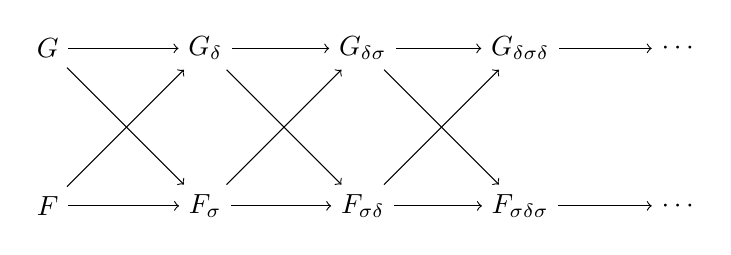
\begin{tikzpicture}
            \node (G) at (-4,1) {\(G\)};
            \node (Gd) at (-2,1) {\(G_\delta\)};
            \node (Gds) at (0,1) {\(G_{\delta \sigma}\)};
            \node (Gdsd) at (2,1) {\(G_{\delta \sigma \delta}\)};
            \node (Gdot) at (4,1) {\(\cdots\)};
            \node (F) at (-4,-1) {\(F\)};
            \node (Fs) at (-2,-1) {\(F_\sigma\)};
            \node (Fsd) at (0,-1) {\(F_{\sigma \delta}\)};
            \node (Fsds) at (2,-1) {\(F_{\sigma \delta \sigma}\)};
            \node (Fdot) at (4,-1) {\(\cdots\)};

            \draw[->] (G) to (Gd); \draw[->] (Gd) to (Gds); \draw[->] (Gds) to (Gdsd); \draw[->] (Gdsd) to (Gdot);
            \draw[->] (F) to (Fs); \draw[->] (Fs) to (Fsd); \draw[->] (Fsd) to (Fsds); \draw[->] (Fsds) to (Fdot);
            \draw[->] (G) to (Fs); \draw[->] (Gd) to (Fsd); \draw[->] (Gds) to (Fsds);
            \draw[->] (F) to (Gd); \draw[->] (Fs) to (Gds); \draw[->] (Fsd) to (Gdsd);
        \end{tikzpicture}
    \end{center}

    此链右侧的极限诱导出了 \(\mathbb{R}^n\) 上的 \ref{definition:Borel set}.
\end{remark}

\begin{definition}[可测函数]
    \setlabel {可测}
    \label {definition:measurable function}
    给出 \(\sigma\) - 代数 \((X,\mathcal{U}),(Y,\mathcal{B})\), 一个函数 \(f:X \to Y\) 称 \(\mathcal{U} - \mathcal{B}\) 可测的,
    若 \(\forall S \in \mathcal{B}(f^{-1}(S) \in \mathcal{U})\).
\end{definition}

\begin{corollary}
    任何连续函数 \(f:X \to Y\) 都是 \(\mathcal{B}(X) - \mathcal{B}(Y)\) 可测的.
\end{corollary}

\begin{definition}[Baire 集]
    \setlabel {Baire 集}
    \label {definition:Baire sets}
    对 \ref{definition:compact topological space} \ref{definition:T2 topological space} 空间 \(X\) 定义其上 Baire 集,
    其由 \ref{definition:compact topological space} \(G_\delta\) 生成.
\end{definition}

\begin{lemma}
    \ref{definition:Baire sets} 是使得所有连续 \(f:X \to \mathbb{R}\) 均可测的最小 \(\sigma\)-代数.

    \begin{proof}
        知 \(X\) \ref{definition:T4 topological space} 可用 \ref{theorem:urysohn's lemma} 构造对应的连续函数.
    \end{proof}
\end{lemma}

\begin{remark}
    若取加法为对称差 \(\Delta\), 乘法为交 \(\cup\), 代数诱导出 \(\mathrm{char} = 2\) 交换幺环结构, 其上亦称理想.
\end{remark}

\subsubsection{测度}

我们可以在习见的实数上做扩展, 得到 \(\mathbb{R} \bigcup \{+\infty,-\infty\}\),
其上可自然的定义加减法与偏序, \(\sup (\varnothing) = - \infty,\inf (\varnothing) = + \infty\).

\begin{definition}
    给出 \(X\) 上一个 \(\sigma\) - 代数 \(\mathcal{A}\), \(\mu: \mathcal{A} \to [0, +\infty]\) 是一个函数, 如果满足对于任意
    不交的 \(A_1, A_2, \cdots \in \mathcal{A}\), 有 \(\mu(\bigcup_{i \in \mathbb{N}}) = \sum_{i \in \mathbb{N}} \mu(A_i)\),
    且 \(\mu(\varnothing) = 0\), 则称 \(\mu\) 是 \(\mathcal{A}\) 上的测度.
\end{definition}

\begin{corollary}
    给出 \(A \subseteq B\), 若有定义则 \(\mu(A) \leq \mu(B)\), 且当 \(\mu (A) < +\infty\) 时, \(\mu(B \setminus A) = \mu(B) - \mu(A)\).

    \begin{proof}
        显然有 \(\mu(B) = \mu(A \cup B) + \mu(B \setminus A) = \mu(A) + \mu(B \setminus A) \geq \mu(A)\).
    \end{proof}
\end{corollary}

\begin{corollary}
    给出 \(A_1, A_2, \cdots \in \mathcal{A}\), 有 \(\mu(\bigcup_{i \in \mathbb{N}} A_i) \leq \sum_{i \in \mathbb{N}} \mu(A_i)\).

    \begin{proof}
        令 \(B_i = A_i \setminus \bigcup_{j<i} B_j\), 有 \(\bigsqcup B_i = \bigcup A_i\), 而 \(\mu (B_i) < \mu (A_i)\).
    \end{proof}
\end{corollary}

\begin{lemma}
    假定 \(A_k \subseteq A_{k+1}\), 则 \(\mu(\bigcup_{i \in \mathbb{N}} A_i) = \lim_{n \to \infty} \mu(A_n)\),
    对称的, 假定 \(A_k \supseteq A_{k+1}\), 且对于某个 \(A_n\), \(\mu(A_n) < \infty\), 则 \(\mu(\bigcap_{i \in \mathbb{N}} A_i) = \lim_{n \to \infty} \mu(A_n)\).

    \begin{proof}
        对于升链, 记 \(A_{-1} = \varnothing\), 注意到 \(\mu(\bigcup_{i \in \mathbb{N}} A_i) = \sum_{i \in \mathbb{N}} \mu(A_i \setminus A_{i-1}) = \lim_{n \to \infty} \sum_{i=1}^n \mu(A_i \setminus A_{i-1}) = \lim_{n \to \infty} \mu(A_n)\).

        对于降链, 假定 \(\mu(A_n) < + \infty\), 对 \(A_n \setminus A_i,A_n \setminus \bigcap_{i \in \mathbb{N}} A_i\) 使用上述结论即可.
    \end{proof}
\end{lemma}

\begin{lemma}
    假定 \(X\) 上的代数 \(\mathcal{A}\) 满足对于其中任意升列 \(A_i \subseteq A_{i+1}\) 均有 \(\bigcup_{i \in \mathbb{N}} A_i\),
    则 \(\mathcal{A}\) 是 \(\sigma\) - 代数.
    
    假定 \(X\) 上的一个 \(\mu:\mathcal{A} \to [0, +\infty]\) 满足对于其中任意升列 \(A_i \subseteq A_{i+1}\) 均有 \(\mu(\bigcup_{i \in \mathbb{N}} A_i) = \lim_{n \to \infty} \mu(A_n)\),
    且 \(\mu(\varnothing) = 0\), 以及有限可加性 \(\mu(\bigcup_{i \in \mathbb{N}} A_i) = \sum_{i \in \mathbb{N}} \mu(A_i)\), 则 \(\mu\) 是测度.

    \begin{proof}
        需验证可数可加性, 只需注意到 \(\bigcup_{i \in \mathbb{N}} A_i = \bigcup_{i \in \mathbb{N}} (\bigcup_{j \leq i} A_j)\).
    \end{proof}
\end{lemma}

\begin{lemma}[容斥原理]
    对于有限集 \(S\) 有 \(\mu(\bigcup S) = \sum_{R \subseteq S} {(-1)}^{\abs{R} - 1} \mu(\bigcap R)\).

    \begin{proof}
        归纳, 对于 \(n = 1\) 有 \(\mu(A) = \mu(A)\), 假定上述式子对 \(n\) 成立, 则对 \(n+1\) 有
        
        \[
            \begin{aligned}
                \mu(\bigcup S) &= \mu(\bigcup (S \setminus \{A\})) + \mu(A) - \mu(\bigcup (S \setminus \{A\}) \cap A) \\
                &= \sum_{R \subseteq S \setminus \{A\}} {(-1)}^{\abs{R} - 1} \mu(\bigcap R) + \mu(A) - \sum_{R \subseteq S \setminus \{A\}} {(-1)}^{\abs{R} - 1} \mu(\bigcap R \cap A) \\
                &= \sum_{R \subseteq S} {(-1)}^{\abs{R} - 1} \mu(\bigcap R)
            \end{aligned}
        \]
    \end{proof}
\end{lemma}

\begin{definition}
    \setlabel {有限}
    \label {definition:finite measure}
    一个测度 \(\mu\) 是有限的, 若 \(\mu(X) < +\infty\).
\end{definition}

\subsubsection{外测度}

\begin{definition}[外测度]
    一个 \(X\) 上的外测度是 \(\mu^\ast : \mathcal{P} (X) \to [0, +\infty]\), 满足

    \begin{enumerate}
        \item \(\mu^\ast(\varnothing) = 0\)
        \item \(A \subseteq B \implies \mu^\ast(A) \leq \mu^\ast(B)\)
        \item \(\mu^\ast(\bigcup_{i \in \mathbb{N}} A_i) \leq \sum_{i \in \mathbb{N}} \mu^\ast(A_i)\)
    \end{enumerate}
\end{definition}

上述定义蕴含有限并, 只需考察 \(\varnothing\) 即可.

\begin{definition}[\(\mu^\ast\) - 可测]
    对于外测度 \(\mu^\ast\), 若对于任意 \(A \subseteq X\) 有 \(\mu^\ast(A) = \mu^\ast(A \cap E) + \mu^\ast(A \setminus E)\), 则称 \(E\) 是 \(\mu^\ast\) - 可测的.
\end{definition}

\begin{definition}[零测]
    \(\mu^\ast\) - 零测集是指外测度为零的集合.
\end{definition}

\begin{lemma}
    \(\mu^\ast\) - 零测集总是 \(\mu^\ast\) - 可测的.

    \begin{proof}
        对于任意集合 \(A,B\) 总是成立 \(\mu^\ast(A) \leq \mu^\ast(A \cap B) + \mu^\ast(A \setminus B)\), 只需证明 \(\mu^\ast(A) \geq \mu^\ast(A \cap B) + \mu^\ast(A \setminus B)\),
        只需注意到 \(\mu^\ast(A) = \mu^\ast(B) + \mu^\ast(A) \geq \mu^\ast(A \cap B) + \mu^\ast(A \setminus B)\).
    \end{proof}
\end{lemma}

\begin{definition}
    对于外测度 \(\mu^\ast\), 记全体 \(\mu^\ast\) - 可测集为 \(\mathcal{M} (\mu^\ast)\), 其是 \(\sigma\) - 代数,
    且 \(\mu^\ast\) 在 \(\mathcal{M} (\mu^\ast)\) 上的限制是测度, 有时记作 \(\mu\).

    \begin{proof}
        显然有 \(\varnothing \in \mathcal{M} (\mu^\ast)\) 且 \(\mu^\ast (\varnothing) = 0\),
        依可测定义, \(S\) 是 \(\mu^\ast\) - 可测的当且仅当 \(X \setminus S\) 亦是 \(\mu^\ast\) - 可测的, 只需考察可数不交并.

        对于有限的情况, 归纳, 对一元情况显然有 \(\mu^\ast(A) = \mu^\ast(A \cap B) + \mu^\ast(A \setminus B)\), 假定任意不交且 
        有限个 \(\mu^\ast\) 可测的 \(B_i\), 总是有 \(\mu^\ast(A) = \sum_{i=1}^{n} \mu^\ast (A \cap B_i) + \mu^\ast (A \setminus \bigcup_{i=1}^{n} B_i)\),
        则对于 \(n+1\) 个不交集 \(B_i\), 有 \(\mu^\ast(A) = \sum_{i=1}^{n} \mu^\ast (A \cap B_i) + \mu^\ast (A \setminus \bigcup_{i=1}^{n} B_i) = \sum_{i=1}^{n+1} \mu^\ast (A \cap B_i) + \mu^\ast (A \setminus \bigcup_{i=1}^{n+1} B_i)\).

        对上述式子希望延伸到 \(n \to \infty\) 的情况, 注意到对于任意 \(n\) 有不等式 \(\mu^\ast(A) \geq \sum_{i=1}^{n} \mu^\ast (A \cap B_i) + \mu^\ast (A \setminus \bigcup_{i=1}^{\infty} B_i)\),
        从而 \(\mu^\ast(A) \geq \sum_{i=1}^{\infty} \mu^\ast (A \cap B_i) + \mu^\ast (A \setminus \bigcup_{i=1}^{\infty} B_i) \geq \mu^\ast(A \cap \bigcup_{i=1}^{\infty} B_i) + \mu^\ast (A \setminus \bigcup_{i=1}^{\infty} B_i)\),
        另一个方向显然成立, 故 \(\bigcup_{i=1}^{\infty} B_i\) 亦是 \(\mu^\ast\) - 可测的.

        同理, 讨论可加性, 对不交的 \(\mu^\ast(\bigcup_{i=1}^\infty B_i)\), 应用 \(\mu^\ast\) - 可测性,
        归纳可证 \(\mu^\ast (\bigcup_{i=1}^{\infty} B_i) = \sum_{i=1}^{n} \mu^\ast (B_i) + \mu^\ast (\bigcup_{i=n}^{\infty} B_i)\),
        令 \(n \to \infty\) 给出不等式 \(\mu^\ast (\bigcup_{i=1}^{\infty} B_i) \geq \sum_{i=1}^{\infty} \mu^\ast (B_i)\),
        另一个方向由外测度性质给出, 故其满足可数可加性, 说明其是测度.
    \end{proof}
\end{definition}

\subsubsection{Lebesgue 测度}

\begin{definition}[Lebesgue 外测度]
    \setlabel {Lebesgue 外测度}
    \label {definition:Lebesgue outer measure}
    定义 \(\mathbb{R}\) 上的 Lebesgue 外测度, 令 \(\mathfrak{O} (X)\) 为全体包含 \(X\) 的开集构成的集合族, 其中元素均为可数或有限个不交的开区间,
    记作 \(\bigcup \{(a_i, b_i): i \in I\}\), 则定义 \(\lambda^\ast: \mathcal{P} (\mathbb{R}) \to [0, +\infty]\) 为

    \[
        \lambda^\ast (A) := \inf (\sum_{i \in I} (b_i - a_i): \bigcup \{(a_i, b_i): i \in I\} \in \mathfrak{O} (X))
    \]

    \begin{proof}
        逐条验证, 首先 \(\mu^\ast (\varnothing) = 0\) 显然, 对于 \(A \subseteq B\) 有 \(\mathfrak{O} (A) \supseteq \mathfrak{O} (B)\),
        于是 \(\mu^\ast (A) \leq \mu^\ast (B)\), 对于求并集, 考察 \(\abs{I} < \infty\), 容易证明:

        \[
            (a,b) = \bigcup_{i \in I} (a_i, b_i) \implies b - a \leq \sum_{i \in I} (b_i - a_i)
        \]


        依赖开集均为 \(F_\sigma\), 我们考察闭集 \([a + \varepsilon/2,b - \varepsilon/2] \subseteq (a,b)\), 其有有限子覆盖, 
        而可以取, 于是上述不等式对无限情况仍然成立, 且若 \(a,b\) 其一发散, 右侧级数亦发散,

        选取 \(P_i \in \mathfrak{O} (A_i)\), 则 \(\bigcup_{i \in \mathbb{N}} P_i \in \mathfrak{O} (\bigcup_{i \in \mathbb{Z}} A_i)\),
        只需证明对区间的合成 \((a,b) \subseteq \bigcup_{i} (a_i,b_i)\) 有:

        \[
            b - a \leq \sum_{i} (b_i - a_i)
        \]
    \end{proof}
\end{definition}

\begin{definition}
    同理亦定义 \(\mathbb{R}^n\) 上的 Lebesgue 外测度, 记集合 \(R = \{\prod_{i=1}^{n} (a_i,b_i)\}\),
    令 \(\mathfrak{O} (X) = \{S \subseteq R : \abs{S} < \aleph_1 \land X \in \bigcup S\}\), 定义 \(\lambda^\ast : \mathcal{P} (\mathbb{R}^n) \to [0, +\infty]\) 为

    \[
        \lambda^\ast (X) := \inf (\sum_{i \in I} \prod_{j=1}^{n} (b_{i,j} - a_{i,j}): \bigcup \{\prod_{i=1}^{n} (a_{i,j},b_{i,j}) : i \in I\} \in \mathfrak{O} (X))
    \]

    \begin{proof}
        注意到可数集的可数并可数, 均显然.
    \end{proof}
\end{definition}

\begin{corollary}
    两个 \(\mathbb{R}\) 上诱导出的 \ref{definition:Lebesgue outer measure} 是一样的.
\end{corollary}

\begin{lemma}
    \(\mathbb{R}\) 上的 \ref{definition:Lebesgue outer measure} 映区间为其长度.
\end{lemma}

\begin{corollary}
    任何 \ref{definition:Borel set} 都是 \(\lambda^\ast\) - 可测的.

    \begin{proof}
        \(\mathbb{R}^\nu\) 是 \ref{definition:lindelof topological space}, 所以只需要对开方块证明其 \(\lambda^\ast\) - 可测,
        只需将两个开方块的交和差写成开方块并集的可数交即可.
    \end{proof}
\end{corollary}

\begin{lemma}
    对于 \(\lambda\) 可测集 \(E\), 其测度为含 \(E\) 开集的测度的下确界,
    也为 \(E\) 内 \ref{definition:compact topological space} 集的测度的上确界.

    \begin{proof}
        前者基于 \ref{definition:Lebesgue outer measure} 的定义, 则取 \ref{definition:compact topological space} 集列 \(C_i \subseteq C_{i+1}\),
        使得 \(\bigcup C_i = \mathbb{R}^\nu\), 我们考察 \(E \cap C_i\) 的测度, 注意到 \(\lambda^\ast (C_i) = \lambda^\ast (C_i \cap E) + \lambda^\ast (C_i \setminus E)\),
        考察包含 \(C_i \setminus E\) 的开集的测度的下确界, 其等同于包含于 \(E \cap C_i\) 的紧集的测度的上确界, 注意到 \(C_i\) 是 \ref{definition:compact topological space}, 故 \(C_i\) 闭, 
        是 \ref{definition:Borel set}, 于是 \(\lambda (E) = \lim_{i \to \infty} \lambda (E \cap C_i)\), 即证明了后者.
    \end{proof}
\end{lemma}

\begin{remark}
    \ref{definition:Lebesgue outer measure} 具有空间平移对称性, 也即变换 \(v \mapsto a+v\) 保持测度和 \(\lambda^\ast\) 可测性质.
\end{remark}

\begin{lemma}
    不是所有 \(\mathbb{R}\) 子集都是 \(\lambda^\ast\) - 可测的.

    \begin{proof}
        我们在 \([0,1)\) 上考虑, 择定 \((\mathbb{R},+)/\mathbb{Q}\), 选取其一组在 \([0,1)\) 上的代表元 \(S\),
        我们证明 \(S\) 是不可测的, 若否, 依赖平移对称性, 对有理数 \(r \in [0,1)\), 集 \((S \cap [0,1-r)) + r\) 亦是可测的,
        集 \(S \cap [1-r,1) + r - 1\) 亦是可测的, 令 \(\lambda (S) = k\), 则 \(\lambda ((S \cap [0,1-r) + r) \cup (S \cap [1-r,1) + r - 1)) = k\),
        而 \(r\) 遍历 \([0,1) \cap \mathbb{Q}\) 时, 上述 \((S \cap [0,1-r) + r) \cup (S \cap [1-r,1) + r - 1)\) 不交的遍历 \([0,1)\),
        而 \(\lambda ([0,1)) = 1\), 不论 \(k\) 是否为 \(0\), 都矛盾.
    \end{proof}
\end{lemma}

\subsubsection{累积分布函数, Cantor 集}

\begin{definition}[累积分布函数]
    \setlabel {累积分布函数}
    \label {definition:cumulative distribution function}
    令 \(\mu\) 是 \((\mathbb{R},\mathcal{B} (\mathbb{R}))\) 上的测度, 定义累积分布函数 \(F_\mu : \mathbb{R} \to \mathbb{R}\) 为:

    \[
        F_\mu (x) := \mu((-\infty,x])
    \]

    则 \(F_\mu\) 是有界, 不减, 且右连续的.

    \begin{proof}
        只需证明对右连续的论断, 只需注意到 \(F_\mu (x+h) = F_\mu (x) + \mu((x,x+h])\), 只需注意到 \(\bigcap_{h \in \mathbb{R}_{>0}} (x,x+h] = \varnothing\).
    \end{proof}
\end{definition}

\begin{remark}
    由于有界不减有左极限 \(F_\mu(b) - \lim_{x \to b^{-}} F_\mu (x) = \mu(\{b\})\).

    另一方面 \(\lim_{x \to -\infty} F_\mu (x) = 0\), 因为 \(\bigcap_{n \in \mathbb{N}} (-\infty,-n] = \varnothing\).
\end{remark}

\begin{lemma}
    有界不减右连续且 \(\lim_{x \to \infty} f = 0\) 的函数 \(f\) 总是可以表为某个测度的累积分布函数.

    \begin{proof}
        定义 \(f(+\infty) = \lim_{x \to \infty} f(x), f(-\infty) = 0\), 改变上述对 \ref{definition:Lebesgue outer measure} 的定义,
        可以令 \(\mu^\ast (A) = \inf (\sum_{i \in I} f(b_i) - f(a_i): \bigcup \{(a_i, b_i): i \in I\} \in \mathfrak{O} (X))\),
        寻同样的思路可证其确为外测度, 且 \ref{definition:Borel set} 可测并给出 \(F_{\mu^\ast} = f\). 
    \end{proof}
\end{lemma}

\begin{definition}[Cantor 集]
    \setlabel {Cantor 集}
    \label {definition:Cantor set}
    定义 Cantor 集 \(C\) 为 \([0,1]\) 上的闭集, 递归定义为:

    \[
        C_0 = [0,1], C_{n+1} = \{x \in [0,1]:3x \in C_{n} \lor 3x - 2 \in C_{n}\}
    \]

    定义 \(C = \bigcap_{n \in \mathbb{N}} C_n\).
\end{definition}

\begin{lemma}
    \ref{definition:Cantor set} 是 \(\mathbb{R}\) 上的不可数 \(\lambda^\ast\) - 零测集.

    \begin{proof}
        构造开覆盖 \(U_0 = (-0.1,1.1), U_{n+1} = \{x \in (-0.1,1.1):3x \in U_n \lor 3x - 2 \in U_n\}\), 其诱导出极限 \(\lim_{n \to \infty} 1.2 \times {(2/3)}^{-n} = 0\).
    \end{proof}
\end{lemma}

\begin{corollary}
    \ref{definition:Cantor set} 有空内部, 且所有点都是其极限点.
\end{corollary}

\begin{definition}[Cantor 函数]
    \setlabel {Cantor 函数}
    \label {definition:Cantor function}
    定义 Cantor 函数 \(c: [0,1] \to [0,1]\) 为:

    \[
        c(\sum_{n=1}^{\infty} \frac{a_n}{3^n}) = \sum_{n=1}^{m} \frac{a_n}{2^{n+1}} + \frac{1}{2^{m+1}}, m = \max \{n: a_n \neq 1\}, a_n \in \{0,1,2\}
    \]
\end{definition}

\begin{corollary}
    \ref{definition:Cantor function} 是 \ref{definition:cumulative distribution function}, 对应的测度仅在 \ref{definition:Cantor set} 上非零.
\end{corollary}

\begin{corollary}
    \ref{definition:Cantor function} 连续, 且在 \ref{definition:Cantor set} 外导数为零, \(c(1) - c(0) = 1\).
\end{corollary}

\begin{lemma}
    \ref{definition:Cantor set} 同胚于 \(\{0,1\}^{\mathbb{N}}\).

    \begin{proof}
        利用 \ref{definition:Cantor set} 的定义, 注意到 \(3x,3x-2\) 不能同时在 \(C_n\) 中, 于是可以对 \(C_n:n \in \mathbb{Z}_{>0}\) 构造 \(F_n\),
        为 \(F_n(x) := \begin{cases}
            0 & 3x \in C_n \\
            1 & 3x - 2 \in C_n
        \end{cases}\), 粘合得到 \((F_1,F_2,\cdots) : C \to \{0,1\}^{\mathbb{N}}\).
    \end{proof}
\end{lemma}

\begin{lemma}
    有同胚 \(C^{m} \to C\), 其中 \(m \in \mathbb{N} \cup \{\aleph_0\}\).

    \begin{proof}
        只需注意到基数等式 \(\aleph_0 \times m = \aleph_0\).
    \end{proof}
\end{lemma}

\begin{lemma}
    存在从 \ref{definition:Cantor set} 到 \([0,1]\) 的连续满射.

    \begin{proof}
        即 \ref{definition:Cantor function}.
    \end{proof}
\end{lemma}

\begin{corollary}
    存在从 \ref{definition:Cantor set} 到 \ref{definition:hilbert cube} 的连续满射.
\end{corollary}

\begin{lemma}
    对 \({\{0,1\}}^{\mathbb{N}}\) 中非空闭集 \(A\), 存在 \({\{0,1\}}^{\mathbb{N}} \to A\) 的连续满射.

    \begin{proof}
        归纳构造 \(f_i : {\{0,1\}}^{i}\), 令 \(f_0 = \varnothing\), 假定业已构造 \(f_n\) 我们来构造 \(f_{n+1}\), 
        假定 \((f_n(x) \cup \{(n,x_{n+1})\}) \in \{a \upharpoonright_{[n]}:a \in A\}\),
        令 \(f_{n+1}(x) = f_n(x) \cup \{(n+1,x_{n+1})\}\), 若否则令 \(f_{n+1}(x) = f_n(x) \cup \{(n+1,1-x_{n+1})\}\).

        粘合 \(f_n\) 得到 \(f : {\{0,1\}}^{\mathbb{N}} \to A\), \(f({\{0,1\}}^{\mathbb{N}}) \subseteq A\) 基于 \(A\) 闭, 此映射满基于 \(\forall x \in A (f(x) = x)\),
        此映射连续基于对于任意基中的开集, 只需考察有限个指标, 则其原像亦无需考察该有限指标之外的指标.
    \end{proof}
\end{lemma}

\begin{theorem}[Alexandroff-Hausdorff]
    任意 \ref{definition:compact topological space} 度量空间 \(X\), 均存在连续函数 \(\phi:C \to X\) 使得 \(\phi(C) = X\),
    其中 \(C\) 是 \ref{definition:Cantor set}.

    \begin{proof}
        嵌入 \ref{definition:hilbert cube}.
    \end{proof}
\end{theorem}

\subsubsection{完备性}

\begin{definition}[完备性]
    一个测度 \(\mu\) 是完备的, 若对于任意 \(\mu\) - 零测集 \(N\), 有 \(\forall A \subseteq N (\mu(A) = 0)\).
\end{definition}

\begin{remark}
    若 \(B\) 包含于一个 \(\mu\) - 零测集, 则 \(B\) 称 \(\mu\) - 可略的.
\end{remark}

\begin{definition}[完备化]
    \setlabel {完备化}
    \label {definition:the completion of a measure}
    给出一个测度 \(\mu\), 定义于 \(X\) 上 \(\sigma\) - 代数 \(\mathcal{A}\), 定义其完备化 \(\mathcal{A}_\mu := \{A \subseteq X : \exists E,F \in \mathcal{A} (E \subseteq A \subseteq F \land \mu(F \setminus E) = 0)\}\),
    也称 \(\mathcal{A}_\mu\) 中的元素可测, 其上可自然的继承 \(\mu\) 的测度, 记作 \(\overline{\mu}\).

    \begin{proof}
        假定有 \(A_1 \subseteq E \subseteq B_1,A_2 \subseteq F \subseteq B_2\), 且 \(\mu(B_1 \setminus A_1) = \mu(B_2 \setminus A_2) = 0\),
        则 \(\mu(B_1) = \mu(A_1) \leq \mu(B_2) = \mu(A_2) \leq \mu(B_1)\), 故 \(\overline{\mu}\) 唯一.

        可数并和补集的性质只需注意到 \(A_1 \subseteq E_1 \subseteq B_1\), 则 \(\bigcup_{i \in \mathbb{N}} A_i \subseteq \bigcup_{i \in \mathbb{N}} E_i \subseteq \bigcup_{i \in \mathbb{N}} B_i\),
        以及 \(A \subseteq E \subseteq B\) 则 \(X \setminus B \subseteq X \setminus E \subseteq X \setminus A\).
    \end{proof}
\end{definition}

\begin{definition}
    给出一个测度 \(\mu\) 定义在 \(X\) 上的 \(\sigma\) - 代数 \(\mathcal{A}\) 上, 定义其对应的内测度 \(\mu_\ast : \mathcal{P} (X) \to [0, +\infty]\) 和外测度 \(\mu^\ast : \mathcal{P} (X) \to [0, +\infty]\) 为:

    \[
        \begin{aligned}
            \mu_\ast (A) &:= \sup \{\mu(B) : B \in \mathcal{A} \land B \subseteq A\} \\
            \mu^\ast (A) &:= \inf \{\mu(B) : B \in \mathcal{A} \land A \subseteq B\}
        \end{aligned}
    \]
\end{definition}

\begin{lemma}
    给定测度 \(\mu\), 若 \(\mu^\ast (A) < + \infty\), 则 \(\mu_\ast (A) = \mu^\ast (A)\) 当且仅当 \(A \in \mathcal{A}_{\mu}\).

    \begin{proof}
        对测度有限集, 注意到若 \(A \subseteq B\) 则 \(\mu(A) = \mu (B) \iff \mu(B \setminus A) = 0\).
    \end{proof}
\end{lemma}

\begin{lemma}
    上述定义出的 \(\mu^\ast\) 是外测度.

    \begin{proof}
        只需逐条验证不等式, 首先 \(\mu^\ast (\varnothing) = 0\) 显然, 其次 \(A \subseteq B\), 蕴含 \(B \subseteq S \implies A \subseteq S\), 
        于是 \(\mu^\ast (A) \leq \mu^\ast (B)\), 同理当无限并时, 假设 \(A_i \subseteq U_i\), 则 \(\bigcup_{i \in \mathbb{N}} A_i \subseteq \bigcup_{i \in \mathbb{N}} U_i\).
    \end{proof}
\end{lemma}

\begin{corollary}
    \ref{definition:Lebesgue outer measure} 是在 \((\mathbb{R}^d,\mathcal{B} (\mathbb{R}^d))\) 上限制的 \ref{definition:the completion of a measure}.
\end{corollary}

\subsubsection{正规性}

\begin{definition}[正规]
    \setlabel {正规}
    \label {definition:regular measure}
    令 \(\mathcal{A} \supseteq \mathcal{B} (\mathbb{R}^\nu)\) 是 \(\sigma\) - 代数,
    称 \(\mathcal{A}\) 上的测度 \(\mu\) 是正规的, 若对于任意 \ref{definition:compact topological space},
    都有 \(\mu(K) < +\infty\), 且对于任意集 \(A\), \(\mu(A)\) 为包含 \(A\) 的开集的测度的下确界, 对于任意开集 \(U\), \(\mu(U)\) 为 \(U\) 子集的 \ref{definition:compact topological space} 集的测度的上确界.
\end{definition}

\begin{lemma}
    \((\mathbb{R}^\nu,\mathcal{B} (\mathbb{R}^\nu))\) 上的有限测度总是 \ref{definition:regular measure}.

    \begin{proof}
        先在矩形 \({[-n,n]}^\nu\) 内讨论, 有界闭集都 \ref{definition:compact topological space}, 利用对 \({[-n,n]}^\nu\) 的补即可, 令 \(n \to \infty\) 就证明了所需结论.
    \end{proof}
\end{lemma}

\subsubsection{Dynkin 类}

\begin{definition}[Dynkin 类]
    \setlabel {Dynkin 类}
    \label {definition:Dynkin class}
    令 \(\mathcal{D}\) 是 \(\mathcal{P} (X)\) 的子集族, 称 \(\mathcal{D}\) 是 Dynkin 类 (或 d - 系统), 若

    \begin{enumerate}
        \item \(X \in \mathcal{D}\)
        \item \((A,B \in \mathcal{D} \land A \subseteq B) \implies B \setminus A \in \mathcal{D}\)
        \item \((A_i \in \mathcal{D} \land A_i \subseteq A_{i+1}) \implies \bigcup_{i \in \mathbb{N}} A_i \in \mathcal{D}\)
    \end{enumerate}
\end{definition}

\begin{definition}[\(\pi\) - system]
    \setlabel {\(\pi\) - 系统}
    \label {definition:pi system}
    令 \(\mathcal{P}\) 是 \(\mathcal{P} (X)\) 的子集族, 称 \(\mathcal{P}\) 是 \(\pi\) - 系统, 
    若 \(\forall A,B \in \mathcal{P} (A \cap B \in \mathcal{P})\).
\end{definition}

\begin{lemma}
    给出一个 \ref{definition:pi system} \(\mathcal{C}\), 其生成的 \(\sigma\) - 代数就是其生成的 \ref{definition:Dynkin class}.

    \begin{proof}
        我们证明其交均在其生成的 \ref{definition:Dynkin class} \(\mathcal{D}\) 中, 构造 \(\mathcal{D}_1 = \{A \in \mathcal{D} : (\forall B \in \mathcal{C}) A \cap B \in \mathcal{D}\}\),
        \(\mathcal{D}_1\) 是 \ref{definition:Dynkin class} 因为

        \[
            \begin{aligned}
                X \cap B &= B \in \mathcal{D} \\
                (A \setminus C) \cap B &= (A \cap B) \setminus (C \cap B) \in \mathcal{D} \\
                (\bigcup_{i \in \mathbb{N}} A_i) \cap B &= \bigcup_{i \in \mathbb{N}} (A_i \cap B) \in \mathcal{D}
            \end{aligned}
        \]

        又 \(\mathcal{C} \subseteq \mathcal{D}_1\) 源自于 \ref{definition:pi system} 的定义, 而 \(\mathcal{D}_1 \subseteq \mathcal{D}\), 故 \(\mathcal{D} = \mathcal{D}_1\).
        然后定义 \(\mathcal{D}_2 = \{A \in \mathcal{D} : (\forall B \in \mathcal{D}) A \cap B \in \mathcal{D}\}\), 依赖 \(\mathcal{D} = \mathcal{D}_1\) 有 \(\mathcal{C} \subseteq \mathcal{D}_2\), 
        且 \(\mathcal{D}_2\) 是 \ref{definition:Dynkin class} 证明同上.

        故 \(\mathcal{D} = \mathcal{D}_2\), 即 \(\mathcal{D}\) 保有限交, 而 \(A \cup B = X \setminus (X \setminus A \cap X \setminus B)\), 于是 \(\mathcal{D}\) 亦保有限并,
        可数并基于 \(\bigcup_{i \in \mathbb{N}} A_i = \bigcup_{i \in \mathbb{N}} \bigcup_{j=0}^{i} A_j\), 故 \(\mathcal{D}\) 是 \(\sigma\) - 代数.
    \end{proof}
\end{lemma}

\begin{corollary}
    假设 \(\mathcal{C}\) 是 \ref{definition:pi system}, \(\mu,\nu\) 是 \((X,\sigma(\mathcal{C}))\) 上的测度,
    满足 \(\mu(X) = \nu(X) < +\infty\), 且 \(\mu,\nu\) 在 \(\mathcal{C}\) 上一致, 则 \(\mu = \nu\).

    \begin{proof}
        \(\{A \in \sigma(\mathcal{C}) : \mu(A) = \nu(A)\}\) 是 \ref{definition:Dynkin class}, 且包含 \(\mathcal{C}\), 故包含 \(\sigma(\mathcal{C})\).
    \end{proof}
\end{corollary}

\subsection{积分}

\subsubsection{\(\mathbb{R}\) 上积分}

业已给出可测函数的定义 \ref{definition:measurable function}, 愿在其上建立有关积分的理论, 我们先从实数开始.

\begin{remark}
    我们给出 \((X,\mathcal{A})\) 上的测度 \(\mu\), 记全体 \(\mathcal{A} - \mathcal{B} (\mathbb{R})\) 可测函数构成的集合为 \(\mathcal{M}\),
    其中非负的记作 \(\mathcal{M}_{\geq 0}\).
\end{remark}

\begin{remark}
    记 \(A\) 的特征函数为 \(\chi_A (x) := \begin{cases}
        1 & x \in A \\
        0 & x \notin A
    \end{cases}\).
\end{remark}

\begin{definition}
    一个函数称简单函数若其可写作 \(\sum_{i=0}^{n} a_i \chi_{A_i}\), 其中 \(A_i\) 两两不交, \(a_i \in \mathbb{R}\), 也即值域有限.
\end{definition}

\begin{definition}[积分]
    对于形如 \(f = \sum_{i=0}^{n} a_i \chi_{A_i}\) 的非负简单函数, 其中 \(A_i\) 两两不交, 我们定义其积分为 \(\int f \dd \mu := \sum_{i=0}^{n} a_i \mu(A_i)\).

    \begin{proof}
        假定 \(\sum_{i=0}^{n} a_i \chi_{A_i} = \sum_{j=0}^{m} b_j \chi_{B_j}\), 依赖不交的性质知道 \(A_i \cap B_j \neq \varnothing \implies a_i = b_j\),
        故 \(\sum_{i=0}^{n} a_i \mu(A_i) = \sum_{i=0}^{n} \sum_{j=0}^{m} a_i \mu(A_i \cap B_j) = \sum_{i=0}^{n} \sum_{j=0}^{m} b_j \mu(A_i \cap B_j) = \sum_{j=0}^{m} b_j \mu(B_j)\).
    \end{proof}
\end{definition}

\begin{lemma}
    给出 \(\alpha \geq 0\), 与 \(f = \sum_{i=1}^{n} f_i \chi_{A^f_i},g = \sum_{i=1}^{m} g_i \chi_{A^g_i}\) 则有积分公式:

    \[
        \begin{aligned}
            \int \alpha f \dd \mu &= \alpha \int f \dd \mu \\
            \int (f+g) \dd \mu &= \int f \dd \mu + \int g \dd \mu \\
            \forall x \in X (f(x) \leq g(x)) &\implies \int f \dd \mu \leq \int g \dd \mu
        \end{aligned}
    \]

    \begin{proof}
        逐条验证, 首先 \(\alpha f = \sum \alpha f_i \chi_{A^f_i}\), 其次 \(f = \sum_{i=1}^{n} \sum_{j=1}^{m} f_i \chi_{A^f_i \cap A^g_j}, g = \sum_{i=1}^{n} \sum_{j=1}^{m} g_j \chi_{A^f_i \cap A^g_j}\),
        于是 \(\int \alpha f \dd \mu = \sum \alpha f_i \mu(A^f_i) = \alpha \sum f_i \mu(A^f_i) = \alpha \int f \dd \mu\), \(\int (f+g) \dd \mu = \sum (f_i + g_j) \mu(A^f_i \cap A^g_j) = \int f \dd \mu + \int g \dd \mu\),
        最后当 \(f \leq g\) 时, 有 \(A^f_i \cap A^g_j \neq \varnothing \implies f_i \leq g_j\), 故 \(\int f \dd \mu = \sum_{i=1}^{n} \sum_{j=1}^{m} f_i \mu(A^f_i \cap A^g_j) \leq \sum_{i=1}^{n} \sum_{j=1}^{m} g_j \mu(A^f_i \cap A^g_j) = \int g \dd \mu\).
    \end{proof}
\end{lemma}

\begin{lemma}
    给出不减非负函数列 \(f_n = \sum_{i=1}^{m_n} f_{n,i} \chi_{A_i^n}\), 给出非负函数 \(f = \sum_{i=1}^{m} a_i \chi_{A_i}\) 使得 \(\forall x \in X (\lim_{n \to \infty} f_n(x) = f(x))\), 则有:

    \[
        \lim_{n \to \infty} \int f_n \dd \mu = \int f \dd \mu
    \]

    \begin{proof}
        显然有 \(\int f_0 \dd \mu \leq \int f_1 \dd \mu \leq \cdots \leq \int f \dd \mu\), 于是 \(\lim_{n \to \infty} \int f_n \dd \mu = \sup_{n \in \mathbb{N}} \int f_n \dd \mu \leq \int f \dd \mu\),
        只需证 \(\lim_{n \to \infty} \int f_n \dd \mu \geq \int f \dd \mu\), 由 \(f = \sum_{i=1}^{m} a_i \chi_{A_i}\), 任取 \(0 < \varepsilon < 1\), 令 \(A_{i,n} = \{x \in X : f_n(x) \geq a_i (1 - \varepsilon)\}\),
        令 \(g_n = \sum_{i=1}^{m} (a_i (1 - \varepsilon)) \chi_{A_{i,n}}\), 有 \(g_n \leq f_n\), 于是 \(\int g_n \dd \mu \leq \int f_n \dd \mu\), 
        另一方面 \(\bigcup_n A_{i,n} = A_i\), 故 \(\lim_{n \to \infty} \mu (A_{i,n}) = \mu (A_i)\), 故 \(\lim_{n \to \infty} \int f_n \dd \mu \geq \lim_{n \to \infty} \int g_n \dd \mu \geq (1 - \varepsilon) \int f \dd \mu\), 
        依赖 \(\varepsilon\) 任意性有 \(\lim_{n \to \infty} \int f_n \dd \mu \geq \int f \dd \mu\).
    \end{proof}
\end{lemma}

依赖上述两个引理, 终可给出非负可测函数的积分的定义.

\begin{definition}[积分]
    \label {definition:integral on nonnegative measurable function}
    任意给出 \(\mathcal{M}_{\geq 0}\) 中非负可测函数 \(f\), 定义其积分为 \(\int f \dd \mu := \sup \{\int g \dd \mu : g = \sum_{i=1}^{n} g_i \chi_{A^g_i} \in \mathcal{M}_{\geq 0}, g \leq f\}\).
\end{definition}

\begin{remark}
    显然, \(\sum_{i=1}^{n} a_i \chi_{A_i}\) 总是非负可测函数.
\end{remark}

\begin{lemma}
    给出 \(\alpha \geq 0\), 与 \(f,g \in \mathcal{M}_{\geq 0}\) 则有积分公式:

    \[
        \begin{aligned}
            \int \alpha f \dd \mu &= \alpha \int f \dd \mu \\
            \int (f+g) \dd \mu &= \int f \dd \mu + \int g \dd \mu \\
            \forall x \in X (f(x) \leq g(x)) &\implies \int f \dd \mu \leq \int g \dd \mu
        \end{aligned}
    \]
\end{lemma}

\begin{lemma}
    给出不减列 \(f_n = \sum_{i=1}^{m_n} f_{n,i} \chi_{A_i^n}\) 使得 \(\forall x \in X (\lim_{n \to \infty} f_n(x) = f(x))\), 则有:

    \[
        \lim_{n \to \infty} \int f_n \dd \mu = \int f \dd \mu
    \]

    \begin{proof}
        对 \(g\) 取 \(\min (f_n,g)\) 即可.
    \end{proof}
\end{lemma}

\begin{definition}[积分]
    \label {definition:integral on measurable function}
    任意给出 \(\mathcal{M}\) 中可测函数 \(f\), 定义 \(f^{+} := \max (f,0), f^{-} := \max (-f,0)\), 假设 \(f^{+},f^{-}\) 的积分有限, 则称 \(f\) 可积,
    定义其积分为 \(\int f \dd \mu := \int f^{+} \dd \mu - \int f^{-} \dd \mu\).
\end{definition}

\begin{lemma}
    令 \(\alpha > 0\), \(f,g\) 为实值可积函数, 则 \(\alpha f, f+g\) 亦可积, 且有积分公式:

    \[
        \begin{aligned}
            \int \alpha f \dd \mu &= \alpha \int f \dd \mu \\
            \int (f+g) \dd \mu &= \int f \dd \mu + \int g \dd \mu \\
            \forall x \in X (f(x) \leq g(x)) &\implies \int f \dd \mu \leq \int g \dd \mu
        \end{aligned}
    \]
\end{lemma}

\begin{corollary}
    \(f\) 可积当且仅当 \(\abs {f}\) 可积, 此时 \(\abs {\int f \dd \mu} \leq \int \abs {f} \dd \mu\).
\end{corollary}

\begin{definition}[Lebesgue 积分]
    \setlabel {Lebesgue 积分}
    \label {definition:Lebesgue integral}
    以 \ref{definition:Lebesgue outer measure} 诱导出的测度建立的积分称为 Lebesgue 积分.
\end{definition}

\begin{lemma}
    给出 \([0,1]\) 上连续函数 \(f\), 则 \(f\) 的 \ref{definition:Riemann-Stieltjes integral} 与 \ref{definition:Lebesgue integral} 相等.

    \begin{proof}
        建立以 \(0,1/2^k,2/2^k,\cdots,1\) 为分割的分段阶梯函数列, 逐点收敛于 \(f\), 故其积分收敛于 \ref{definition:Lebesgue integral}, 依赖 \(f\) 的一致连续性, 知其积分收敛于 \ref{definition:Riemann-Stieltjes integral},
        故两者相等.
    \end{proof}
\end{lemma}

\subsubsection{几乎处处成立}

\begin{definition}
    给定一个关于 \(X\) 上某点的性质 \(P\). 其称为 \(\mu\) - 几乎处处成立, 若存在 \(\mu\) - 零测集 \(N\) 使得 \(P\) 在 \(X \setminus N\) 上成立.
\end{definition}

\begin{lemma}
    若实值函数 \(f,g\) 有 \(\mu\) - 几乎处处 \(f = g\), \(\mu\) 完备, 那么 \(f\) 可测则 \(g\) 可测.
\end{lemma}

\begin{lemma}
    若实值函数列 \(f_n\) 有 \(\mu\) - 几乎处处逐点收敛于 \(f\), \(\mu\) 完备, 那么每个 \(f_n\) 可测则 \(f\) 可测.

    \begin{proof}
        对开集 \(U\) 在 \(X \setminus N\) 上有 \(f^{-1} (U) = \bigcup_{n \in \mathbb{N}} \bigcap_{m \geq n} f_m^{-1} (U)\).
    \end{proof}
\end{lemma}

\begin{lemma}
    若 \(f\) 取值于 \([0,+\infty]\) 且可测, 则存在非负简单函数增列 \(f_n\) 取值于 \([0,+\infty]\) 逐点收敛于 \(f\).

    \begin{proof}
        对 \(k \in [n 2^n]\) 定义 \(A_{n,k} = \{x \in X : \frac{k-1}{2^n} \leq f(x) < \frac{k}{2^n}\}\), 其可测基于 \(f\) 可测,
        令 \(f_n = \sum_{k=1}^{n 2^n} \frac{k-1}{2^n} \chi_{A_{n,k}}\).
    \end{proof}
\end{lemma}

\begin{lemma}
    给出 \((X,\mathcal{A},\mu)\), 若 \([-\infty,+\infty]\) 值函数 \(f\) 在 \(\mathcal{A}_\mu\) 上可测, 则存在 \(f_0,f_1\) 以 \([-\infty,\infty]\) 为值使得 \(\forall x \in X (f_0(x) \leq f(x) \leq f_1(x))\), 且 \(\mu\) - 几乎处处 \(f_0 = f_1\).

    \begin{proof}
        假定 \(f\) 为值非负的简单函数, 有 \(f = \sum_{i=1}^{n} a_i \chi_{A_i}\), 假使 \(C_i \subseteq A_i \subseteq B_i\), 使得 \(\mu(B_i \setminus C_i) = 0\), 令 \(f_0 = \sum_{i=1}^{n} a_i \chi_{C_i}, f_1 = \sum_{i=1}^{n} a_i \chi_{B_i}\), 有 \(\mu\) - 几乎处处 \(f_0 = f_1\)
        且 \(f_0 \leq f \leq f_1\).

        对于一般情况, 分离 \(f^+,f^-\) 并用简单函数逼近即可.
    \end{proof}
\end{lemma}

\begin{lemma}
    若 \(\int f \dd \mu,\int g \dd \mu\) 存在且 \(\mu\) - 几乎处处 \(f = g\), 则 \(\int f \dd \mu = \int g \dd \mu\).

    \begin{proof}
        令 \(h(x) = \begin{cases}
            + \infty & f(x) \neq g(x) \\
            0 & f(x) = g(x)
        \end{cases}\), 有 \(\int h \dd \mu = 0\), 故 \(\int f \dd \mu \leq \int g \dd \mu + \int h \dd \mu = \int g \dd \mu\).
    \end{proof}
\end{lemma}

\begin{lemma}
    令 \(f\) 在 \([0,+ \infty]\) 中取值, 令 \(A_t = \{x \in X : f(x) \geq t\}\), 则
    
    \[
        \mu (A_t) \leq \frac{1}{t} \int_{A_t} f \dd \mu \leq \frac{1}{t} \int f \dd \mu
    \]
\end{lemma}

\begin{example}
    给出 \(\mathbb{R}\) 上的非负有界函数 \(f\) 使得 \(\int f \dd \lambda = 1\), 则有不等式:

    \[
        \int_{\abs{x} \geq \varepsilon} f \geq \frac{1}{\varepsilon^2} \int f x^2 \dd \lambda
    \]
\end{example}

\subsubsection{若干极限定理}

\begin{theorem}[单调收敛定理]
    给出取值 \([0,+\infty]\) 的非负函数列 \(f_n\) 不减, 且 \(f = \lim f_n\) \(\mu\) - 几乎处处成立, 则 \(\lim \int f_n \dd \mu = \int f \dd \mu\).

\end{theorem}

\subsection{其他测度}

\subsubsection{Hausdorff 测度}
\subsubsection{Radon 测度}

\begin{definition}[Radon 测度]
    \setlabel {Radon 测度}
    \label {definition:Radon measure}
    给出 \ref{definition:regular measure} \(\mu_\alpha\) 在 \((X_\alpha,\mathcal{A}_\alpha)\) 上的测度,
    如果满足 \(\mu_\alpha(X_\alpha) = 1\), 则在 \(\prod X_\alpha\) 上有唯一的测度 \(\mu\), 使得给出 \(S_{\alpha_1} \subseteq \mathcal{A}_{\alpha_1}, S_{\alpha_2} \subseteq \mathcal{A}_{\alpha_2}, \cdots, S_{\alpha_n} \subseteq \mathcal{A}_{\alpha_n}\), 有:

    \[
        \mu(\pi^{-1} (S_{\alpha_1} \times S_{\alpha_2} \times \cdots \times S_{\alpha_n})) = \prod_{i=1}^{n} \mu_{\alpha_i} (S_{\alpha_i})
    \]
\end{definition}

\subsubsection{Haar 测度}

